\section{Results}
\label{sec:results}

\begin{figure}[b]
  \centering
  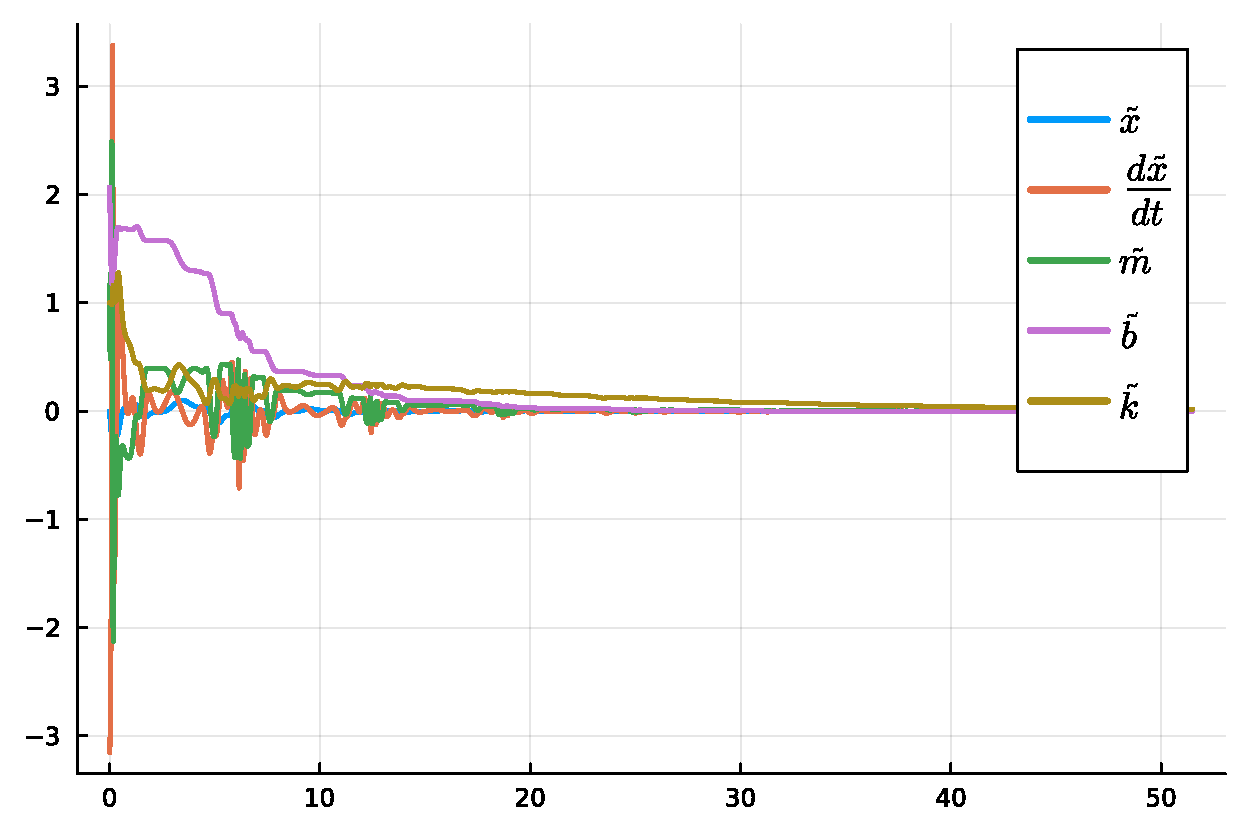
\includegraphics[width=0.5\textwidth]{./figures/adaptationrule2.pdf}
  \caption{Simulation showing the convergence of the system state and parameter
  estimates.}
  \label{fig:adaptation}
\end{figure}

In Figure~\ref{fig:adaptation}, we plot the response of the system to the
control and adaptation laws~(\ref{eq:ctrl_law}, \ref{eq:param_update}),
implemented in simulation. The constants that are used are as follows: $(A, n,
\varphi) = (\nicefrac{3}{10}, 3, 0^\circ)$, $\Gamma = \text{diag}{(1, 1,
\nicefrac{1}{10})}$ and $(c, \lambda) = (1, 4)$. The real mass, damping and
stiffness of the system are $(m, b, k) = (0.665, 1.819, 0)$ and their estimates
start at $(\hat{m}, \hat{b}) = (-\nicefrac{1}{2}, -\nicefrac{1}{4}, -1)$.
